\chapter{Derivaciones Matemáticas Detalladas}\label{app:math_derivations}

% =====================Estilo de página================================
\pagestyle{fancy}
\fancyhf{} % Limpia todos los campos de encabezado y pie de página
% \fancyhead[LE]{\nouppercase{\textit{\rightmark}}} % Sección en páginas pares (izquierda)
% \fancyhead[RO]{\nouppercase{\textit{\rightmark}}} % Sección en páginas impares (derecha)
\fancyhead[RE]{\nouppercase{\hfill \textbf{\leftmark}}} % Capítulo en páginas impares (izquierda)
\fancyhead[LO]{\nouppercase{\textbf{\leftmark} \hfill}} % Capítulo en páginas pares (derecha)
\fancyfoot[LE]{\nouppercase{\thepage \hfill {Pressure Distribution Inside Nucleons in a Tsallis-MIT Bag Model}}} % Pie de página en páginas pares
\fancyfoot[RO]{\nouppercase{{Pressure Distribution Inside Nucleons in a Tsallis-MIT Bag Model} \hfill \thepage}} % Pie de página en páginas impares
% =====================================================================

\section{Derivaciones detalladas del gas de gluones}
\label{app:BE_derivation}

\subsection{Densidad de estados y función de partición}
Para gluones (bosones sin masa), la relación energía-momento es:
\begin{equation}
\epsilon = pc = \hbar c k
\end{equation}

La densidad de estados en el espacio de fases:
\begin{equation}
g(\epsilon)d\epsilon = g_G \frac{V \epsilon^2 d\epsilon}{\pi^2 (hc)^3}
\end{equation}
donde $g_G = 16$ (8 tipos de gluones $\times$ 2 proyecciones de espín).

\subsection{Integrales fundamentales}
Las cantidades termodinámicas requieren evaluar integrales de la forma:
\begin{equation}
I_n = \int_0^\infty \frac{\epsilon^n d\epsilon}{e^{\beta\epsilon} - 1}
\end{equation}

Mediante el cambio $x = \beta\epsilon$:
\begin{equation}
I_n = \frac{1}{\beta^{n+1}} \int_0^\infty \frac{x^n dx}{e^x - 1} = \frac{\Gamma(n+1)\zeta(n+1)}{(k_B T)^{n+1}}
\end{equation}

Valores particulares:
\begin{align}
\int_0^\infty \frac{x^2 dx}{e^x - 1} &= 2\zeta(3) \approx 2.404 \\
\int_0^\infty \frac{x^3 dx}{e^x - 1} &= \frac{\pi^4}{15} \approx 6.494
\end{align}

\subsection{Energía del sistema (Ecuación \ref{eq-BE-Etotalgluons})}
La energía total se obtiene de:
\begin{equation}
E_G = \frac{g_G V}{\pi^2 (hc)^3} \int_0^\infty \frac{\epsilon^3 d\epsilon}{e^{\beta\epsilon} - 1} = \frac{g_G V}{\pi^2 (hc)^3} \frac{\pi^4 (k_B T)^4}{15}
\end{equation}

Y usando unidades naturales\footnote{\textbf{Nota sobre unidades naturales}: En las ecuaciones finales se ha tomado $\hbar = c = k_B = 1$, con $h = 2\pi$ para consistencia con la literatura \gls{qcd}.}

\begin{equation}
E_G = g_G \frac{\pi^2}{30} V T^4
\end{equation}

\subsection{Presión (Ecuación \ref{eq-BE-Pgluons})}
Partiendo de la función de partición:
\begin{equation}
\ln \Xi = -\frac{g_G V}{\pi^2 (hc)^3} \int_0^\infty \epsilon^2 \ln(1 - e^{-\beta\epsilon}) d\epsilon
\end{equation}

Integrando por partes:
\begin{equation}
\ln \Xi = \frac{g_G V}{3\pi^2 (hc)^3 \beta} \int_0^\infty \frac{\epsilon^3 d\epsilon}{e^{\beta\epsilon} - 1} = \frac{g_G V \pi^2 (k_B T)^3}{90 (hc)^3}
\end{equation}

La presión resulta:
\begin{equation}
P_G = \frac{k_B T}{V} \ln \Xi = \frac{g_G \pi^2 (k_B T)^4}{90 (hc)^3}
\end{equation}

Confirmando la relación ultrarrelativista:
\begin{equation}
P_G = \frac{1}{3} \frac{E_G}{V}
\end{equation}

\subsection{Entropía (Ecuación \ref{eq-BE-Sgluons})}
A partir del potencial gran canónico:
\begin{equation}
S_G = -\left( \frac{\partial \phi}{\partial T} \right)_{V,\mu} = \frac{4}{3} \frac{E_G}{T} = g_G \frac{4\pi^2}{90} V T^3
\end{equation}

\subsection{Demostración de $\mu = 0$ para gluones}
El potencial químico debe anularse porque:
\begin{equation}
N_G(T,V,0) = \frac{g_G V}{\pi^2 (hc)^3} \int_0^\infty \frac{\epsilon^2 d\epsilon}{e^{\beta\epsilon} - 1} \propto T^3
\end{equation}

No hay restricción en el número de gluones (pueden crearse/aniquilarse libremente), por lo que $\mu_G = 0$ en equilibrio termodinámico.

% Los niveles de energía de un bosón en un gas ideal de \gls{be} ultrarrelativista están dados por:

% \begin{equation}
% {\epsilon}_{k} = cp = \hbar c k,
% \end{equation}

% donde $p$ es la magnitud del momento de las partículas del gas y $k$ la magnitud del vector de onda. La función de partición para este sistema es:

% \begin{equation}\label{eq-partfunc}
% {\Xi}^{\mathrm{BE}}\left(T,V,\mu\right) = \prod_{k=1}^{\infty}\frac{1}{1-\xi {e}^{-\beta {\epsilon}_{k}}},
% \end{equation}

% donde $\beta = \frac{1}{{k}_{\mathrm{B}}T}$, y ${\xi} = {e}^{\beta \mu}$ es la fugacidad del gas, $T$ es la temperatura del gas, $V$ el volumen del gas y $\mu$ el potencial químico del gas. El número de partículas promedio en cada estado de energía ${\epsilon}_{k}$ se calcula a través de la ecuación:

% \begin{equation}\label{eq-avg-numb-parts}
% \left\langle {n}_{k} \right\rangle = -\frac{1}{\beta} \frac{\partial}{\partial {\epsilon}_{k}} \ln {\Xi}^{\mathrm{BE}}\left.\right|_{\xi,V,{\epsilon}_{i \neq k}},
% \end{equation}

% Las cantidades termodinámicas fundamentales se expresan como:

% \begin{equation}\label{eq-BE-Ntotal}
% N(T,V,\mu) = \sum_k \langle n_k \rangle = \sum_k \frac{1}{{\xi}^{-1}{e}^{\beta{\epsilon}_{k}}-1}
% \end{equation}

% \begin{equation}\label{eq-BE-Etotal}
% E(T,V,\mu) = \sum_k \langle n_k \rangle \epsilon_k = \sum_k \frac{\epsilon_k}{{\xi}^{-1}{e}^{\beta{\epsilon}_{k}}-1}
% \end{equation}

% De tal manera que el número total de partículas promedio y energía se pueden calcular como

% \begin{equation}\label{eq-BE-Ntotal}
% N(T,V,\mu)=\sum_{k}\left\langle {n}_{k} \right\rangle = \sum_{k}\frac{1}{{\xi}^{-1}{e}^{\beta{\epsilon}_{k}}-1}
% \end{equation}

% \begin{equation}\label{eq-BE-Etotal}
% E(T,V,\mu) = \sum_{k}\left\langle {n}_{k} \right\rangle {\epsilon}_{k} = \sum_{k}\frac{{\epsilon}_{k}}{{\xi}^{-1}{e}^{\beta{\epsilon}_{k}}-1}.
% \end{equation}

% Para una gran cantidad de partículas, podemos sustituir la suma por una integral, considerando el número total de estados en el espacio fase clásico tenemos

% \begin{equation}
% \begin{split}
% \Sigma &= \int \frac{\mathrm{d}^{3}r \mathrm{d}^{3}p}{{h}^{3}} \\ 
% & = V\int \frac{4\pi {p}^{2} \mathrm{d}p}{{h}^{3}} \\
% & = \frac{4\pi V}{{h}^{3}} \int_{0}^{\infty} {p}^{2} \mathrm{d} p 
% \end{split}
% \end{equation}

% Usando la relación ${\epsilon}_{k} = cp$ obtenemos

% \begin{equation}\label{eq-totalestados}
% \Sigma = \frac{4\pi V}{(hc)^{3}} \int_{0}^{\infty} {\epsilon}^{2} \mathrm{d} \epsilon
% \end{equation} 

% De esta forma, sustituyendo \eqref{eq-totalestados} en \eqref{eq-BE-Ntotal} y \eqref{eq-BE-Etotal}, obtenemos

% \begin{equation}\label{eq-BE-Ntotalint}
% N(T,V,\mu) = \frac{4\pi V}{(hc)^{3}} \int_{0}^{\infty} \frac{{\epsilon}^{2} \mathrm{d} \epsilon}{{\xi}^{-1} {e}^{\beta \epsilon} - 1}
% \end{equation}

% \begin{equation}\label{eq-BE-Etotalint}
% E(T,V,\mu) = \frac{4\pi V}{(hc)^{3}} \int_{0}^{\infty} \frac{{\epsilon}^{3} \mathrm{d} \epsilon}{{\xi}^{-1} {e}^{\beta \epsilon} - 1}
% \end{equation}

% Dado que tratamos con partículas sin masa, es posible tener infinitas partículas con energía ${\epsilon}_{0}=0$. De esta manera, el potencial químico $\mu$ debe ser cero pues es posible crear infinitas partículas con energía $0$ sin afectar a nuestros resultados puesto que no contribuyen a la energía total del sistema. Así, si $\mu=0$, entonces $\xi = 1$. Y sustituyendo en las ecuaciones \eqref{eq-BE-Ntotalint} y \eqref{eq-BE-Etotalint} obtenemos 

% \begin{equation}\label{eq-BE-Ntotalintnofug}
% N(T,V) = \frac{4\pi V}{(hc)^{3}} \int_{0}^{\infty} \frac{{\epsilon}^{2} \mathrm{d} \epsilon}{{e}^{\beta \epsilon} - 1}
% \end{equation}

% \begin{equation}\label{eq-BE-Etotalintnofug}
% E(T,V) = \frac{4\pi V}{(hc)^{3}} \int_{0}^{\infty} \frac{{\epsilon}^{3} \mathrm{d} \epsilon}{ {e}^{\beta \epsilon} - 1}
% \end{equation}

% Para resolver las integrales, consideramos el cambio de variable $x=\beta \epsilon$, por lo que $\epsilon = \frac{x}{\beta}$ y así $\mathrm{d}\epsilon = \frac{\mathrm{d}x}{\beta}$ y así, entonces 

% \begin{equation}\label{eq-BE-Ntotalintnofug-x}
% N(T,V) = \frac{4\pi V}{(hc)^{3}} \frac{1}{{\beta}^{3}}\int_{0}^{\infty} \frac{{x}^{2} \mathrm{d} x}{{e}^{x} - 1}
% \end{equation}

% \begin{equation}\label{eq-BE-Etotalintnofug-x}
% E(T,V) = \frac{4\pi V}{(hc)^{3}} \frac{1}{{\beta}^{4}} \int_{0}^{\infty} \frac{{x}^{3} \mathrm{d} x}{ {e}^{x} - 1}
% \end{equation}

% Con lo cual, obtenemos las funciones especiales ${g}_{n}(\xi)$ con $0 \leq \xi \leq 1$ tales que

% \begin{equation}\label{eq-g-xi}
% {g}_{n}(\xi) = \frac{1}{\Gamma(n)} \int_{0}^{\infty} \frac{{x}^{n-1} \mathrm{d}x}{{\xi}^{-1}{e}^{x}-1}
% \end{equation}

% Tal que las integrales de \eqref{eq-BE-Ntotalintnofug-x} y \eqref{eq-BE-Etotalintnofug-x} se vuelven

% \begin{equation}\label{eq-sol-int-N}
% \int_{0}^{\infty} \frac{{x}^{2} \mathrm{d} x}{ {e}^{x} - 1} = \Gamma(3) {g}_{3}(1)
% \end{equation}

% \begin{equation}\label{eq-sol-int-E}
% \int_{0}^{\infty} \frac{{x}^{3} \mathrm{d} x}{ {e}^{x} - 1}= \Gamma(4) {g}_{4}(1)
% \end{equation}

% Sustituyendo las ecuaciones \eqref{eq-sol-int-N} y \eqref{eq-sol-int-E} en \eqref{eq-BE-Ntotalintnofug-x} y \eqref{eq-BE-Etotalintnofug-x}, respectivamente, y usando la propiedad ${g}_{n}(1) = \zeta(n)$, con $\zeta(n)$ representando la función zeta de Rienamann, se obtiene

% \begin{equation}\label{eq-BE-Ntotalintreduced1}
% N(T,V) = \frac{4\pi V}{(hc)^{3}} \frac{1}{{\beta}^{3}}\Gamma(3) \zeta(3)
% \end{equation}

% \begin{equation}\label{eq-BE-Etotalintreduced1}
% E(T,V) = \frac{4\pi V}{(hc)^{3}} \frac{1}{{\beta}^{4}} \Gamma(4) \zeta(4)
% \end{equation}

% Ya que $\Gamma(n-1) = n!$ y $\zeta(4) = \frac{{\pi}^{4}}{90}$ se llega a

%  \begin{equation}\label{eq-BE-Ntotalintreduced2}
% N(T,V) = 8\pi V \left(\frac{{k}_{\mathrm{B}}T}{hc} \right)^{3} \zeta(3)
% \end{equation}

% \begin{equation}\label{eq-BE-Etotalintreduced2}
% E(T,V) = \frac{8\pi V}{(hc)^{3}} \left({k}_{\mathrm{B}} T \right)^{4} \frac{{\pi}^{4}}{30}
% \end{equation}

% Y usando unidades naturales $\hbar={k}_{\mathrm{B}}=c=1$ y $h=2\pi \hbar = 2\pi$, así entonces

%  \begin{equation}\label{eq-BE-Ntotalintreduced3}
% N(T,V) = \frac{1}{{\pi}^{2}} \zeta(3)V{T}^{3}
% \end{equation}

% \begin{equation}\label{eq-BE-Etotalintreduced3}
% E(T,V) = \frac{{\pi}^{2}}{30} V{T}^{4}
% \end{equation}

% Finalmente, dado que hay tres componentes independientes de la carga de color, y consecuentemente $3 \times 3 - 1$ generadores de $SU(3)$, hay 8 diferentes tipos de gluones, y como cada gluón tiene dos proyecciones de espín, el factor de degeneración corresponde a ${g}_{G} = 8 \times 2 = 16$. Por lo tanto, pasamos a que las expresiones para el número total de gluones y la energía total de gluones como un gas ideal de \gls{be} ultrarrelativista son

%  \begin{equation}\label{eq-BE-Ntotalgluons}
% {N}_{G}(T,V) = \frac{{g}_{G}}{{\pi}^{2}} \zeta(3)V{T}^{3}
% \end{equation}

% \begin{equation}\label{eq-BE-Etotalgluons}
% {E}_{G}(T,V) = {g}_{G}\frac{{\pi}^{2}}{30} V{T}^{4}
% \end{equation}

% Para calcular la contribución de presión debido a los gluones, partimos de la función de partición ${\Xi}^{BE}$ y el potencial macrocanónico o potencial gran canónico $\phi$

% \begin{equation}\label{eq-BE-P1}
% \begin{split}
% \phi = -PV  & = -{k}_{\mathrm{B}} T \ln {\Xi}^{BE} \\ 
% \Rightarrow P & = \frac{{k}_{\mathrm{B}}T}{V} \ln {\Xi}^{BE}
% \end{split}
% \end{equation}

% Calculando el logaritmo de la función de partición \eqref{eq-partfunc} se tiene

% \begin{equation}
% \ln {\Xi}^{BE} = - \sum_{k=1}^{\infty} \ln\left(1 - \xi{e}^{-\beta {\epsilon}_{k}}\right)
% \end{equation}

% Nuevamente ocupamos el hecho de que son estados energéticos tan cercanos y tal cantidad de partículas en distintos estados energéticos, podemos sustituir la suma por una integral, usando el número total de estados \eqref{eq-totalestados} y el hecho de que no hay potencial químico ($\mu=0 \Rightarrow \xi=1$) para obtener

% \begin{equation}
% \ln {\Xi}^{BE} = - \frac{4\pi V}{(hc)^{3}} \int_{0}^{\infty} {\epsilon}^{2} \ln \left(1 - {e}^{-\beta\epsilon} \right) \mathrm{d} \epsilon
% \end{equation}

% Realizando la integral por partes tendremos

% \begin{equation}
% \begin{split}
% \ln {\Xi}^{BE} & = - \frac{4\pi V}{(hc)^{3}} \left[ \left. \frac{1}{3} {\epsilon}^{3} \ln \left( 1 - {e}^{-\beta \epsilon}\right) \right|_{0}^{\infty} - \frac{1}{3} \beta \int_{0}^{\infty} \frac{{\epsilon}^{3} \mathrm{d}\epsilon}{{e}^{\beta \epsilon} - 1} \right] \\ 
% & = \frac{4\pi V}{(hc)^{3}} \frac{kT}{3} \int_{0}^{\infty} \frac{{\epsilon}^{3} \mathrm{d} \epsilon}{{e}^{-\beta \epsilon} - 1}
% \end{split}
% \end{equation}

% Resolviendo la integral, de la misma forma que con la ecuación \eqref{eq-BE-Etotalintnofug}, usando \eqref{eq-sol-int-E} y simplificando se llega a que la presión ejercida por un gas de partículas ultrarrelativistas tipo \gls{be}, usando la expresión \eqref{eq-BE-P1}, está dada como

% \begin{equation}\label{eq-BE-P2}
% P= \frac{1}{3} \frac{E}{V}
% \end{equation}

% Y dado que existen ${g}_{G}$ estados degenerados para la energía de los gluones, entonces, la presión correspondiente a los gluones es, usando \eqref{eq-BE-Etotalgluons},

% \begin{equation}\label{eq-BE-Pgluons}
% {P}_{G} = {g}_{G} \frac{{\pi}^{2}}{90}{T}^{4}
% \end{equation}

% Como cálculo final, hallamos la entropía a partir del potencial gran canónico por medio de la relación

% \begin{equation}\label{eq-BE-Entropy}
% \begin{split}
% \phi &= E-TS-\mu N = -PV, \\
% \Rightarrow S & = \frac{1}{T} \left(E+PV- \mu N \right)
% \end{split}
% \end{equation}

% Sustituyendo la ecuación \eqref{eq-BE-P2} en \eqref{eq-BE-Entropy} y considerando $\mu=0$, la entropía del sistema es

% \begin{equation}\label{eq-BE-S}
% S = \frac{4}{3} \frac{E}{T}
% \end{equation}

% Y tomando en cuenta que tratamos con la energía de gluones \eqref{eq-BE-Etotalgluons}, la entropía del gas de gluones está dado como

% \begin{equation}\label{eq-BE-Sgluons}
% {S}_{G} = 4{g}_{G} \frac{{\pi}^{2}}{90}V{T}^{3}.
% \end{equation}

\section{Derivaciones detalladas del gas compuesto de quarks y antiquarks}
\subsection{Relación energía-momento y espectro de partículas}
Para partículas con masa despreciable ($m \ll \|\overrightarrow{p}\|/c$), la energía se aproxima a:
\begin{equation}
\epsilon = \sqrt{p^2c^2 + m^2c^4} \approx pc \quad \text{(ultrarrelativista)}
\end{equation}

El número de estados cuánticos en el elemento de volumen $d^3p$ es:
\begin{equation}
g(\epsilon) d\epsilon = g_Q \frac{V \epsilon^2 d\epsilon}{(hc)^3 \pi^2}
\end{equation}
donde $g_Q = 12$ (2 spines $\times$ 3 colores $\times$ 2 sabores).

\subsection{Función de partición y número de partículas}
Para quarks ($+$) y antiquarks ($-$), la función de partición es:
\begin{equation}
\ln \Xi = \sum_{\epsilon} \left[ \ln\left(1 + e^{-\beta(\epsilon-\mu)}\right) + \ln\left(1 + e^{-\beta(\epsilon+\mu)}\right) \right]
\end{equation}

El número promedio de partículas se obtiene de $\langle N_\pm \rangle = \partial \ln \Xi / \partial (\beta \mu_\pm)$:
\begin{equation}
N_\pm = \int_0^\infty \frac{g(\epsilon) d\epsilon}{e^{\beta(\epsilon \mp \mu)} + 1}
\end{equation}

\subsection{Cálculo del exceso neto de quarks (Ecuación \ref{eq-FD-Excedente})}
Transformando las integrales con $x = \beta \epsilon$:
\begin{align}
N &= N_+ - N_- = \frac{g_Q V}{(hc)^3 \pi^2} \left[ \int_0^\infty \frac{\epsilon^2 d\epsilon}{e^{\beta(\epsilon-\mu)} + 1} - \int_0^\infty \frac{\epsilon^2 d\epsilon}{e^{\beta(\epsilon+\mu)} + 1} \right] \nonumber \\
&= \frac{g_Q V (kT)^3}{\pi^2 (hc)^3} \left[ \int_{-\beta\mu}^\infty \frac{(x + \beta\mu)^2 dx}{e^x + 1} - \int_{\beta\mu}^\infty \frac{(x - \beta\mu)^2 dx}{e^x + 1} \right]
\end{align}

Desarrollando las integrales (ver Sección \ref{sec:FD_integrals}):
\begin{equation}
N = \frac{g_Q V}{6\pi^2} \left( \pi^2 \mu T^2 + \mu^3 \right)
\end{equation}

\subsection{Energía del sistema (Ecuación \ref{eq-FD-Energy})}
La energía total incluye contribuciones de quarks y antiquarks:
\begin{align}
E &= \int_0^\infty \frac{\epsilon \cdot g(\epsilon) d\epsilon}{e^{\beta(\epsilon-\mu)} + 1} + \int_0^\infty \frac{\epsilon \cdot g(\epsilon) d\epsilon}{e^{\beta(\epsilon+\mu)} + 1} \nonumber \\
&= \frac{g_Q V}{\pi^2 (hc)^3} \left[ \int_0^\infty \frac{\epsilon^3 d\epsilon}{e^{\beta(\epsilon-\mu)} + 1} + \int_0^\infty \frac{\epsilon^3 d\epsilon}{e^{\beta(\epsilon+\mu)} + 1} \right]
\end{align}

Expandiendo en términos de $\beta\mu$:
\begin{equation}
E_Q = g_Q V T^4 \left[ \underbrace{\frac{7\pi^2}{120}}_{\text{térmico}} + \underbrace{\frac{1}{4}\left(\frac{\mu}{T}\right)^2 + \frac{1}{8\pi^2}\left(\frac{\mu}{T}\right)^4}_{\text{químico}} \right]
\end{equation}

\subsection{Presión y entropía}
Usando la relación ultrarrelativista $P = E/3V$:
\begin{equation}
P_Q = \frac{g_Q T^4}{3} \left[ \frac{7\pi^2}{120} + \frac{\mu^2}{4T^2} + \frac{\mu^4}{8\pi^2 T^4} \right]
\end{equation}

Para la entropía, partiendo de $S = (\partial/\partial T)(kT \ln \Xi)$:
\begin{equation}
S_Q = g_Q V T^3 \left[ \frac{7\pi^2}{90} + \frac{1}{6}\left(\frac{\mu}{T}\right)^2 \right]
\end{equation}

\subsection{Detalles de integración}
\label{sec:FD_integrals}
Las integrales tipo Fermi-Dirac se resuelven mediante:
\begin{align}
\int_0^\infty \frac{x^n dx}{e^x + 1} &= \Gamma(n+1)\left(1 - 2^{-n}\right)\zeta(n+1) \\
\int_0^\infty \frac{x dx}{e^x + 1} &= \frac{\pi^2}{12}, \quad \int_0^\infty \frac{x^3 dx}{e^x + 1} = \frac{7\pi^4}{120}
\end{align}

Para integrales con $\mu \neq 0$, se usa la expansión de Sommerfeld:
\begin{equation}
\int_{-\beta\mu}^\infty f(x) \frac{dx}{e^x + 1} \approx \int_0^{\beta\mu} f(x) dx + \frac{\pi^2}{6} f'(0) + \mathcal{O}(e^{-\beta\mu})
\end{equation}

% Las partículas ultrarelativistas tienen una relación energía-momento $\epsilon = \| \overrightarrow{p} \| c$\footnote{De la fórmula general $\epsilon = \sqrt{{p}^{2}{c}^{2} + {m}^{2}{c}^{4}}$, para masa en reposo despreciable.}.

% Hay ciertos bosones con esta relación energía-momento, pero el número de fermiones con masa en reposo despreciable es muy poca. Para casos prácticos, ``despreciable'' significa una masa en reposo del orden de los neutrinos (${m}_{\nu} < 8 $eV). El gas ultrarelativistico de \gls{fd} puede ser visto como un gas caliente de fermiones con masa en reposo no despreciable, esto es, si el momento promedio en el gas es grande comparado con $mc$, es decir, si la energía térmica promedio $kT$ es grande comparada con la masa en reposo.

% A partir de mecánica cuántica relativista, se sabe que uno puede crear pares de partículas y antipartículas (quarks y antiquarks, en nuestro caso) del vacío con un gasto energético de $2m{c}^{2}$. Por lo tanto, no debemos considerar un gas de partículas \gls{fd} solitarias, sino como pares partícula-antipartícula.

% Así, trataremos con una mezcla de dos gases ideales \gls{fd}, entre las cuales, son posibles reacciones ``químicas''.

% La función de partición para un gas ideal de \gls{fd}  está determinada por:

% \begin{equation}
% {\Xi}^{\mathrm{FD}}(T,V,\mu)=\prod_{k=1}^{\infty} \left(1 + \xi {e}^{-\beta {\epsilon}_{k}} \right)
% \end{equation}

% En este caso se considera una mezcla de gases (quarks y antiquarks), entonces la función de partición está dada como

% \begin{equation}
% \Xi\left(T,V,{\mu}_{+},{\mu}_{-}\right) = \prod_{{\epsilon}_{+}} \left(1+ {\xi}_{+}{e}^{-\beta {\epsilon}_{+}} \right) + \prod_{{\epsilon}_{-}} \left(1+ {\xi}_{-}{e}^{-\beta {\epsilon}_{-}} \right)
% \end{equation}

% donde ${\xi}_{+} = {e}^{\beta {\mu}_{+}}$ y ${\xi}_{-} = {e}^{\beta{\mu}_{-}}$ y el signo $+$ corresponde a las partículas mientras que el signo $-$ a las antipartículas. El número promedio de partículas en cada estado de energía se puede calcular usando la ecuación \eqref{eq-avg-numb-parts} y se obtiene

% \begin{equation}\label{eq-FD-NumbParts}
% \left\langle{n}_{k} \right\rangle = \frac{1}{{\xi}^{-1}{e}^{\beta{\epsilon}_{k}} + 1}
% \end{equation}

% por lo que el número total promedio para las partículas se calcularía a través de

% \begin{equation}\label{eq-FD-Tot-Numb-Parts}
% \begin{split}
% {N}_{+}(T,V,{\mu}_{+}) &= \sum_{{\epsilon}_{+}} \left\langle{n}_{{\epsilon}_{+}} \right\rangle\\
% & = \sum_{{\epsilon}_{+}} \frac{1}{{\xi}_{+}^{-1}{e}^{\beta{{\epsilon}}_{+}} + 1}
% \end{split}
% \end{equation}

% Y de manera análoga se obtiene el número total promedio de antipartículas

% \begin{equation}\label{eq-FD-Tot-Numb-Antiparts}
% \begin{split}
% {N}_{-}(T,V,{\mu}_{-}) &= \sum_{{\epsilon}_{-}} \left\langle{n}_{{\epsilon}_{-}} \right\rangle\\
% & = \sum_{{\epsilon}_{-}} \frac{1}{{\xi}_{-}^{-1}{e}^{\beta{{\epsilon}}_{-}} + 1}
% \end{split}
% \end{equation}

% En equilibrio termodinámico el número de promedio de partículas y antipartículas cambia constantemente debido al proceso de creación y aniquilación, por lo que no es conveniente fijar el número de ambas y posteriormente determinar los potenciales químicos. En lugar de ello, se realiza el siguiente análisis a fin de fijar el potencial químico.

% Los cambios $d{N}_{+}$ y $d{N}_{-}$ de los dos números de partículas están relacionados por la relación

% $$
% d{N}_{+} = d{N}_{-}
% $$

% Las reacciones que suceden en el gas de quarks y antiquarks son de la forma

% $$
% q + \bar{q} \rightleftharpoons \, \mathrm{productos \; de \; reacci\acute{o}n} + \Delta E
% $$

% observamos que una antipartícula se crea o aniquila con cada partícula. Además, el resto de las partículas generadas por las reacciones creación-aniquilación no juegan un rol en el gas que estamos considerando de quarks antiquarks. Por esta razón, podemos notar que los potenciales químicos de partículas y antipartículas tienen que ser iguales con signos opuestos, ya que los productos de la reacción no contienen potencial químico,

% \begin{equation}\label{eq-FD-chpot-fug}
% {\mu}_{+} + {\mu}_{-} = 0, \quad {z}_{+}{z}_{-}=1
% \end{equation}

% Los números de partículas ${N}_{+}$ y ${N}_{-}$ no son independientes uno de otro, y por lo tanto no hay dos fugacidades independientes, sino en realidad solo uno. Sin embargo, en vez de ${N}_{+}$ y ${N}_{-}$ uno puede fijar la diferencia $N = {N}_{+} - {N}_{-}$, el excedente de partículas, yaa que no está influenciada por los procesos de creación y aniquilación:

% \begin{equation}\label{eq-FD-ExcedenteNumParts}
% \begin{split}
% N & = {N}_{+} - {N}_{-} \\
% & = \sum_{{\epsilon}_{+} > 0} \frac{1}{{\xi}_{+}^{-1}{e}^{\beta{{\epsilon}}_{+}} + 1} -\sum_{{\epsilon}_{-} > 0} \frac{1}{{\xi}_{-}^{-1}{e}^{\beta{{\epsilon}}_{-}} + 1}
% \end{split}
% \end{equation}

% A partir de esta ecuación, uno determina la fugacidad tomando en cuenta la ecuación \eqref{eq-FD-chpot-fug}. En este sistema, el excedente $N$ de partículas no cambia por creación-aniquilación, pero el número de partículas medio ${N}_{+}$ y ${N}_{-}$ no puede ser controlado.

% \begin{wrapfigure}{l}{0.35\textwidth}
% \centering
% 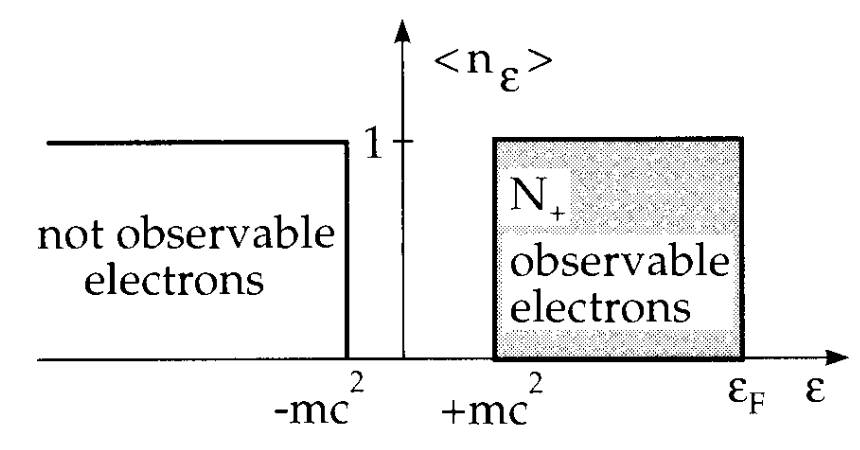
\includegraphics[width=0.35\textwidth]{./Images/ParticleNumberGaswithTnull.png}
% \caption[Número de partículas para un gas de electrones a $T=0$]{\emph{$\left\langle {n}_{k} \right\rangle$ para un gas de electrones a $T=0$}}
% \label{fig: Gas de electrones}
% \end{wrapfigure}

% Para explicar lo anterior, tenemos que considerar el espectro de energía de la ecuación libre de Dirac. En el caso ultrarelativista, $m \rightarrow 0$. En este espectro también hay estados de energía $\epsilon \leq -m {c}^{2}$ además de los estados de energía positiva $\epsilon \geq m{c}^{2}$. Uno puede describir ahora partículas y antipartículas en el espectro simultáneamente, si uno asume que en el vacío, sin partículas, todos los estados de energía negativa continua están ocupadas por electrones (inobservables).

% En esta imagen de partículas (como son los electrones), en el continuo negativo (agujeros) son interpretados como antipartículas.

% Para un gas de electrones con ${N}_{+}$ electrones y una energía de Fermi ${\epsilon}_{\mathrm{FD}} > m{c}^{2}$ tenemos en $T=0$ la situación de la figura \ref{fig: Gas de electrones}.

% Si se aumenta la temperatura del gas de electrones, al principio, los electrones cerca de la energía de Fermi son excitados a estados más altos ${\epsilon} > {\epsilon}_{\mathrm{FD}}$. Esto ocurre en un rango de energía de anchura aproximada $kT$ alrededor de la energía de Fermi.

% Sin embargo, si la temperatura es del orden de $2m{c}^{2}$, más y más electrones de un continuo más bajo pueden ser excitados en estados libres $\epsilon > {\epsilon}_{\mathrm{FD}}$. Estos electrones dejan huecos en el continuo más bajo, que representan positrones observables. El número de electrones observables también se incrementa. La diferencia ${N}_{+} - {N}_{-}$ sin embargo es la misma que antes. La energía negativa de los huecos ${\epsilon}_{\mathrm{huecos}} < - m{c}^{2}$ es simplemente relacionada a la energía positiva del positrón correspondiente como ${\epsilon}_{{e}^{+}} = - {\epsilon}_{\mathrm{hueco}}$.

% El número de electrones y positrones observables puede ser calculado como sigue:

% \begin{equation}\label{eq-FD-NumbPartsAndAntiparts}
% {N}_{+} = \sum_{\epsilon>0} \left\langle {n}_{k} \right\rangle, \quad {N}_{-} = \sum_{\epsilon<0} \left(1 - \left\langle {n}_{k} \right\rangle \right)
% \end{equation}

% donde $\left\langle {n}_{k} \right\rangle$ está dado por \eqref{eq-FD-NumbParts} y ${\mu} = {\mu}_{+}$ como el potencial químico de los electrones (partículas). La expresión para ${N}_{-}$ puede ser transformada como

% \begin{equation}\label{eq-FD-NumbTotAntiparts}
% \begin{split}
% {N}_{-} & = \sum_{\epsilon < 0} \left( 1 - \frac{1}{{\xi}^{-1}{e}^{\beta{\epsilon}} + 1} \right)  \\
% & = \sum_{\epsilon < 0}\frac{{\xi}^{-1}{e}^{\beta \epsilon}}{{\xi}^{-1}{e}^{\beta{\epsilon}} + 1} \\
% & = \sum_{\epsilon<0} \frac{1}{{\xi}{e}^{-\beta{\epsilon}} + 1}
% \end{split}
% \end{equation}

% El espectro de energía de la ecuación libre de Dirac es simétrica alrededor de $\epsilon=0$. Así, uno puede sustituir $\epsilon \rightarrow -{\epsilon}_{-}$ en \eqref{eq-FD-NumbTotAntiparts} y entonces consideramos positrones con energía positiva.

% \begin{equation}
% {N}_{-} = \sum_{{\epsilon}_{-}>0} \frac{1}{{\xi}{e}^{\beta{\epsilon}_{-}}+1}
% \end{equation}

% Y por otro lado ${\xi} = {\xi}_{-}^{-1}$; es decir, ${\mu}_{+} = - {\mu}_{-}$. Ambas interpretaciones llevan a los mismos resultados, pero en algunos casos, la imagen de partícula-hueco de Dirac es más conveniente. Por ejemplo, el exceso de partículas en esta imagen es simplemente

% \begin{equation}
% \begin{split}
% N & = {N}_{+} - {N}_{-} = \sum_{\epsilon > 0} \left\langle {n}_{\epsilon} \right\rangle - \sum_{\epsilon < 0} \left(1 - \left\langle {n}_{\epsilon} \right\rangle \right) \\
% & = \sum_{\epsilon} \left\langle {n}_{\epsilon} \right\rangle  - \sum _{\epsilon < 0} 1 = \sum_{\epsilon} \left\langle {n}_{\epsilon} \right\rangle  - \sum_{\epsilon} \left\langle {n}_{\epsilon} \right\rangle ^{\mathrm{vac}}
% \end{split}
% \end{equation}


% %%%%%%%%%%%%%%%%%%%%%%%%%%%%%%%%%%%%%%%%%%%
% %%%%COMPLETAR EL RESTO DE LA EXPLICACIÓN%%%%%%%
% %%%%%%%%%%%%%%%%%%%%%%%%%%%%%%%%%%%%%%%%%%%


% Ahora procedemos con el cálculo de la presión. Tenemos que reescribir las sumas en la ecuación \eqref{eq-FD-ExcedenteNumParts}

% \begin{equation}
% {g}(\epsilon) = g \frac{4\pi V}{{h}^{3}{c}^{3}} {\epsilon}^{2}
% \end{equation}

% \begin{equation}
% \ln \mathcal{Z} = g \frac{4 \pi V}{{h}^{3}{c}^{3}} \int_{0}^{\infty} {\epsilon}^{2} \, \mathrm{d} \epsilon \left[\ln \left( 1 + {e}^{-\beta \left(\epsilon - \mu \right)} \right) + \ln \left(1 + {e}^{-\beta \left(\epsilon + \mu\right)} \right) \right]
% \end{equation}

% de esta manera, podemos reescribir el número total de partículas 

% \begin{equation}
% N =\frac{4 \pi V}{(hc)^{3}} \left[ \int_{0}^{\infty} \frac{{\epsilon}^{2} \mathrm{d} \epsilon}{{e}^{\beta (\epsilon-\mu)} + 1} - \int_{0}^{\infty} \frac{{\epsilon}^{2} \mathrm{d} \epsilon}{{e}^{\beta (\epsilon+\mu)} + 1} \right] 
% \end{equation}

% Para la primera integral se hace el cambio de variable $x = \beta (\epsilon - \mu)$ por lo que  $\epsilon = \frac{x}{\beta} + \mu$ y $\mathrm{d} \epsilon = \frac{\mathrm{d}x }{\beta} $. Para la segunda, se hace $y = \beta(\epsilon + \mu)$ por lo que  $\epsilon = \frac{y}{\beta} - \mu$ y $\mathrm{d}\epsilon = \frac{\mathrm{d}y}{\beta}$. Y haciendo los respectivos cambios en los límites de integración, se obtiene 

% \begin{equation}\label{eq-FD-int-Numb-Parts-Ints1}
% N = \frac{4 \pi V}{(hc)^{3}} \frac{1}{\beta} \left[ \int_{-\beta \mu}^{\infty} \frac{(\frac{x}{\beta} + \mu)^{2}}{{e}^{x}+1}  \mathrm{d}x - \int_{\beta \mu}^{\infty} \frac{(\frac{y}{\beta} - \mu)^{2}}{{e}^{y}+1}  \mathrm{d}y \right]
% \end{equation}

% Factorizando el término $\beta$ en los numeradores de \eqref{eq-FD-int-Numb-Parts-Ints1} y reacomodando los límites de integración,podemos reescribir

% \begin{equation}\label{eq-FD-int-Numb-Parts-Ints2}
% \begin{split}
% N &= \frac{4 \pi V}{(hc)^{3}} \frac{1}{{\beta}^{3}} \left[\int_{-\beta \mu}^{\infty} \frac{(x + \beta \mu)^{2}}{{e}^{x}+1}  \mathrm{d}x - \int_{\beta \mu}^{\infty} \frac{(y -\beta \mu)^{2}}{{e}^{y}+1}  \mathrm{d}y \right] \\
% & = \frac{4 \pi V}{(hc)^{3}} \frac{1}{{\beta}^{3}} \left[ \int_{-\beta \mu}^{0} \frac{(x + \beta \mu)^{2}}{{e}^{x}+1}  \mathrm{d}x + \int_{0}^{\infty} \frac{(x + \beta \mu)^{2}}{{e}^{x}+1}\mathrm{d}x \right. \\
% & \left. - \int_{\beta \mu}^{0} \frac{(y -\beta \mu)^{2}}{{e}^{y}+1}  \mathrm{d}y  - \int_{0}^{\infty} \frac{(y -\beta \mu)^{2}}{{e}^{y}+1}  \mathrm{d}y  \right]
% \end{split}
% \end{equation}

% Juntando las integrales que van de cero a infinito en \eqref{eq-FD-int-Numb-Parts-Ints2}, y reemplazando $y \rightarrow x$, se tiene

% \begin{equation}\label{eq-FD-int-Numb-Parts-IntsPart1-2}
% \begin{split}
% \int_{0}^{\infty} \frac{(x + \beta \mu)^{2}}{{e}^{x}+1}\mathrm{d}x - \int_{0}^{\infty} \frac{(y -\beta \mu)^{2}}{{e}^{y}+1}  \mathrm{d}y & = \int_{0}^{\infty} \frac{(x +\beta \mu)^{2} - (x -\beta \mu)^{2}}{{e}^{y}+1}  \mathrm{d}y \\
% & = 4\beta \mu \int_{0}^{\infty} \frac{x}{{e}^{x} + 1} \mathrm{d} x.
% \end{split}
% \end{equation}

% Podemos juntar el resto de las integrales si trabajamos una de ellas con un cambio de variable para ajustar los límites integrales a los mismos $y \rightarrow -x$, como

% \begin{equation}
% \begin{split}
% - \int_{\beta \mu}^{0} \frac{(y -\beta \mu)^{2}}{{e}^{y}+1}  \mathrm{d}y & =  \int_{0}^{\beta \mu} \frac{(y -\beta \mu)^{2}}{{e}^{y}+1}  \mathrm{d}y \\
% & = - \int_{0}^{-\beta \mu} \frac{(-x -\beta \mu)^{2}}{{e}^{-x}+1}  \mathrm{d}x \\
% & = \int_{-\beta \mu}^{0} \frac{(x + \beta \mu)^{2}}{{e}^{-x}+1}  \mathrm{d}x
% \end{split}
% \end{equation}

% Y de esta manera

% \begin{equation}\label{eq-FD-int-Numb-Parts-IntsPart2-2}
% \begin{split}
% \int_{-\beta \mu}^{0} \frac{(x + \beta \mu)^{2}}{{e}^{x}+1}  \mathrm{d}x - \int_{\beta \mu}^{0} \frac{(y -\beta \mu)^{2}}{{e}^{y}+1}  \mathrm{d}y & = \int_{-\beta \mu}^{0} \frac{(x + \beta \mu)^{2}}{{e}^{x}+1}  \mathrm{d}x  +  \int_{-\beta \mu}^{0} \frac{(x + \beta \mu)^{2}}{{e}^{-x}+1}  \mathrm{d}x \\ 
% & =  \int_{-\beta \mu}^{0} (x + \beta \mu)^{2} \left[\frac{1}{{e}^{x} + 1} + \frac{1}{{e}^{-x} + 1} \right] \mathrm{d}x \\
% & = \int_{-\beta \mu}^{0} (x + \beta \mu)^{2} \mathrm{d}x
% \end{split}
% \end{equation}

% Dado que en el paréntesis cuadrado de \eqref{eq-FD-int-Numb-Parts-IntsPart2-2}, al multiplicar por ${e}^{x}$ el segundo término, se llega a que los dos términos dentro del paréntesis dan la unidad. De esta manera, el número de partículas, sustituyendo \eqref{eq-FD-int-Numb-Parts-IntsPart1-2} y \eqref{eq-FD-int-Numb-Parts-IntsPart2-2} en \eqref{eq-FD-int-Numb-Parts-Ints2}

% \begin{equation}
% N = \frac{4 \pi V}{(hc)^{3}} \frac{1}{{\beta}^{3}} \left[4\beta \mu \int_{0}^{\infty} \frac{x}{{e}^{x} + 1} \mathrm{d} x + \int_{-\beta \mu}^{0} (x + \beta \mu)^{2} \mathrm{d}x \right]
% \end{equation}

% Haciendo el cambio de variable ${z} = x + \beta \mu$ en la última integral se obtiene

% \begin{equation}\label{eq-FD-int-Numb-Parts-Ints3}
% N = \frac{4 \pi V}{(hc)^{3}} \frac{1}{{\beta}^{3}} \left[4\beta \mu \int_{0}^{\infty} \frac{x}{{e}^{x} + 1} \mathrm{d} x + \int_{0}^{\beta \mu} {z}^{2} \mathrm{d}z \right]
% \end{equation}

% Y de manera análoga a lo que es la función \eqref{eq-g-xi}, tenemos las funciones especiales ${f}_{n}(\xi)$ con $0 \leq \xi \leq 1$:

% \begin{equation}\label{eq-f-xi}
% {f}_{n}(\xi) = \frac{1}{\Gamma(n)} \int_{0}^{\infty} \frac{{x}^{n-1} \mathrm{d}x}{{\xi}^{-1}{e}^{x} + 1}
% \end{equation}

% Entonces la primera integral de \eqref{eq-FD-int-Numb-Parts-Ints3} se vuelve

% \begin{equation}
% \int_{0}^{\infty} \frac{x}{{e}^{x} + 1} \mathrm{d} x = \Gamma(2) {f}_{2}(1) = {f}_{2}(1)
% \end{equation}

% Por último, las funciones ${f}_{n}(\xi)$ cumplen con la propiedad:

% \begin{equation}\label{eq-f-xi=1}
% {f}_{n}(1) = \left(1 - \frac{1}{{2}^{n-1}} \right) \zeta (n)
% \end{equation}

% Usando la ecuación \eqref{eq-f-xi=1} y que $\zeta(2)= \displaystyle \frac{{\pi}^{2}}{6}$ en la primera integral de \eqref{eq-FD-int-Numb-Parts-Ints3}, se obtiene

% \begin{equation}\label{eq-FD-int-Numb-Parts-Ints3-1/2}
% \int_{0}^{\infty} \frac{x}{{e}^{x} + 1} \mathrm{d} x = \frac{{\pi}^{2}}{12}
% \end{equation}

% Y para la segunda integral, se obtiene simplemente

% \begin{equation}\label{eq-FD-int-Numb-Parts-Ints3-2/2}
% \int_{0}^{\beta \mu} {z}^{2} \mathrm{d}z = \frac{(\beta \mu)^{3}}{3}
% \end{equation}

% Sustituyendo \eqref{eq-FD-int-Numb-Parts-Ints3-1/2} y \eqref{eq-FD-int-Numb-Parts-Ints3-2/2} en \eqref{eq-FD-int-Numb-Parts-Ints3} se llega a la expresión

% \begin{equation}
% \begin{split}
% N & = \frac{4 \pi V}{(hc)^{3}} \frac{1}{{\beta}^{3}} \left[4 \beta \mu \frac{{\pi}^{2}}{12} + \frac{(\beta \mu)^{3}}{3} \right] \\
% & = 4 \pi V \left(\frac{kT}{hc} \right)^{3} \left[ \frac{{\pi}^{2}}{3} \left(\frac{\mu}{kT}\right) + \frac{1}{3} \left(\frac{\mu}{kT} \right)^{3} \right]
% \end{split}
% \end{equation}

% Y ahora, analógamente con el gas ideal de \gls{be}, la expresión se reescribe en unidades naturales usando $c=\hbar = {k}_{\mathrm{B}} = 1$ y $h = 2\pi$, y se agrega el factor de degeneración de los quarks ${g}_{Q}$

% \begin{equation}\label{eq-FD-Total-Number-Particles-Quarks}
% {N}_{Q} = \frac{{g}_{Q}}{6} \left[\frac{\mu}{T} + \frac{1}{{\pi}^{2}} \left(\frac{\mu}{T} \right)^{3} \right] V{T}^{3}
% \end{equation}

% El factor de degeneración de los quarks se compone del producto del número de proyecciones de espín (${N}_{s}$), el número de colores, ${N}_{c}$, y el número de sabores, ${N}_{f}$, a consideración ${g}_{G}={N}_{s}{N}_{c}{N}_{f}$. Para este caso, se tienen ${N}_{s}=2$ proyecciones de espín, ${N}_{c}=3$ colores y ${N}_{f}=2$ sabores, $u$ y $d$, dado que bajo este esquema, analizamos materia nuclear ordinaria. Por tanto ${g}_{Q}=12$.

% Para calcular la contribución de los quarks y antiquarks a la energía del sistema, se considera

% \begin{equation}
% E = {E}_{+} + {E}_{-} = \sum_{{\epsilon}_{+}>0} \left\langle{n}_{{\epsilon}_{+}} \right\rangle {\epsilon}_{+} + \sum_{{\epsilon}_{-}>0} \left\langle{n}_{{\epsilon}_{-}} \right\rangle {\epsilon}_{-} 
% \end{equation}

% donde ${E}_{+}$ es la energía de los quarks y ${E}_{-}$ de los antiquarks. Usando la ecuación \eqref{eq-FD-NumbParts}, y la relación entre las fugacidades explicada con anterioridad \eqref{eq-FD-chpot-fug}, podemos establecer que 

% \begin{equation}\label{eq-FD-Quark-Energy-Ints}
% \begin{split}
% E & = \sum_{{\epsilon}_{+} > 0} \frac{{\epsilon}_{+}}{{e}^{\beta({\epsilon}_{+}-\mu)} + 1} + \sum_{{\epsilon}_{-} > 0} \frac{{\epsilon}_{-}}{{e}^{\beta({\epsilon}_{-}+\mu)} + 1} \\
% & \Rightarrow \frac{4{\pi}V}{(hc)^{3}} \left[ \int_{0}^{\infty}  \frac{{\epsilon}^{3} \mathrm{d} \epsilon}{{e}^{\beta({\epsilon}-\mu)} + 1}+ \int_{0}^{\infty}\frac{{\epsilon}^{3} \mathrm{d} \epsilon}{{e}^{\beta({\epsilon}+\mu)} + 1} \right]
% \end{split}
% \end{equation}

% Donde se ha usado el número total de estados en el espacio fase clásico \eqref{eq-totalestados}. A partir de aquí, se procede a hacer el mismo procedimiento que para el cálculo del número total de partículas para resolver las integrales \eqref{eq-FD-Quark-Energy-Ints}, de lo que se llega fácilmente a que 

% \begin{equation}\label{eq-FD-Quark-Energy-Ints2}
% \begin{split}
% E & = \frac{4\pi V}{(hc)^{3}} \frac{1}{{\beta}^{4}} \left[2\int_{0}^{\infty} \frac{{x}^{3}}{{e}^{x} + 1} \mathrm{d}x + 6(\beta \mu)^{2} \int_{0}^{\infty} \frac{x}{{e}^{x}+1} \mathrm{d}x + \int_{-\beta \mu}^{0} \left(x + \beta \mu \right)^{3} \mathrm{d}x \right] \\
% & = \frac{4\pi V}{(hc)^{3}} \frac{1}{{\beta}^{4}} \left[2\int_{0}^{\infty} \frac{{x}^{3}}{{e}^{x} + 1} \mathrm{d}x + 6(\beta \mu)^{2} \int_{0}^{\infty} \frac{x}{{e}^{x}+1} \mathrm{d}x + \int_{0}^{\beta \mu} {z}^{3} \mathrm{d}z \right]
% \end{split}
% \end{equation}

% Donde se ha usado el cambio de variable $z=x+\beta \mu$ para la última integral. Para resolver las primeras integrales, hacemos uso de las funciones \eqref{eq-f-xi}

% \begin{equation}\label{eq-FD-Quark-Energy-Ints-1/3}
% \int_{0}^{\infty} \frac{{x}^{3}}{{e}^{x} + 1} \mathrm{d} x = \Gamma(4){f}_{4}(1) = \frac{7{\pi}^{4}}{120}
% \end{equation}

% La segunda integral se obtuvo con anterioridad \eqref{eq-FD-int-Numb-Parts-Ints3-1/2}, y la tercera se cálcula directamente como

% \begin{equation}\label{eq-FD-Quark-Energy-Ints-3/3}
% \int_{0}^{\beta \mu}{z}^{3} \mathrm{d}z = \frac{(\beta\mu)^{4}}{4}
% \end{equation}

% Así, sustituyendo las ecuaciones \eqref{eq-FD-Quark-Energy-Ints-1/3}, \eqref{eq-FD-int-Numb-Parts-Ints3-1/2} y \eqref{eq-FD-Quark-Energy-Ints-3/3} en \eqref{eq-FD-Quark-Energy-Ints2}, obtenemos

% \begin{equation}
% \begin{split}
% E & = \frac{4\pi V}{(hc)^{3}} \frac{1}{{\beta}^{4}}  \left[2 \left(\frac{7{\pi}^{4}}{120} \right) + 6 (\beta \mu)^{2} \frac{{\pi}^{2}}{12} + \frac{1}{4}(\beta \mu)^{4}\right] \\
% & = \frac{4\pi V}{(hc)^{3}} (kT)^{4} \left[\frac{7{\pi}^{4}}{60} + \frac{{\pi}^{2}}{2} \left(\frac{\mu}{kT} \right)^{2} + \frac{1}{4} \left(\frac{\mu}{kT} \right)^{4}\right]
% \end{split}
% \end{equation}

% Finalmente, usando unidades naturales como con el número de partículas, y agregando el factor de degeneración, obtenemos la energía del gas de quarks - antiquarks

% \begin{equation}\label{eq-FD-Quark-Energy}
% {E}_{Q} = {g}_{Q} \left[\frac{7{\pi}^{2}}{120} + \frac{1}{4} \left(\frac{\mu}{T} \right)^{2} + \frac{1}{8{\pi}^{2}} \left(\frac{\mu}{T} \right)^{4}\right]V{T}^{4}
% \end{equation}

% Para finalizar el cálculo de cantidades termodinámicas en este modelo, calculamos la presión producida por los quarks y antiquarks de manera análoga como con los gluones. La presión está definida por la ecuación \eqref{eq-BE-P1}, entonces para este caso, tenemos la función de partición que está dada como

% \begin{equation}\label{eq-FD-Log-Part-Func}
% \begin{split}
% \ln \Xi &= \sum_{{\epsilon}_{+}} \ln \left(1+{e}^{-\beta({\epsilon}_{+}-\mu)} \right) + \sum_{{\epsilon}_{-}} \ln \left(1+{e}^{-\beta({\epsilon}_{-}+\mu)} \right) \\ 
% & \Rightarrow \frac{4 \pi V}{(hc)^{3}} \left[ \int_{0}^{\infty} {\epsilon}^{2} \ln \left(1 + {e}^{-\beta(\epsilon - \mu)} \right) \mathrm{d}\epsilon + \int_{0}^{\infty} {\epsilon}^{2} \ln \left(1 + {e}^{-\beta(\epsilon + \mu)} \right) \right]
% \end{split}
% \end{equation}

% donde se han reemplazado las sumas por las integrales. Para resolver las integrales, ocupamos integración por partes, para la primera integral tenemos

% \begin{equation}\label{eq-FD-Log-Part-Func-Int1}
% \begin{split}
% \int_{0}^{\infty} {\epsilon}^{2} \ln \left(1 + {e}^{-\beta(\epsilon-\mu)} \right) \mathrm{d} \epsilon & = \left. \frac{{\epsilon}^{3}}{3} \ln \left(1+{e}^{-\beta(\epsilon-\mu)} \right) \right|_{0}^{\infty} + \frac{\beta}{3} \int_{0}^{\infty} \frac{ {\epsilon}^{3} \mathrm{d} \epsilon}{{e}^{\beta(\epsilon - \mu)} + 1} \\
% & = \frac{\beta}{3} \int_{0}^{\infty} \frac{{\epsilon}^{3} \mathrm{d} \epsilon}{{e}^{\beta (\epsilon - \mu)} + 1 }
% \end{split}
% \end{equation}

% En el cual, después de evaluar en los límites en la ecuación \eqref{eq-FD-Log-Part-Func-Int1}, se llega a que se cancela el primer término. Para la segunda integral de \eqref{eq-FD-Log-Part-Func} se procede similarmente y se obtiene

% \begin{equation}\label{eq-FD-Log-Part-Func-Int2}
% \int_{0}^{\infty} {\epsilon}^{2} \ln \left(1 + {e}^{-\beta(\epsilon + \mu)} \right) = \frac{\beta}{3} \int_{0}^{\infty} \frac{{\epsilon}^{3} \mathrm{d} \epsilon}{{e}^{\beta (\epsilon + \mu)} + 1 }
% \end{equation}

% Y, sustituyendo las ecuaciones \eqref{eq-FD-Log-Part-Func-Int1} y  \eqref{eq-FD-Log-Part-Func-Int2} en \eqref{eq-FD-Log-Part-Func}, obtenemos 

% \begin{equation}
% \ln \Xi = \frac{4\pi V }{(hc)^{3}} \frac{\beta}{3} \left[\int_{0}^{\infty} \frac{{\epsilon}^{3} \mathrm{d} \epsilon}{{e}^{\beta (\epsilon - \mu)} + 1 } + \int_{0}^{\infty} \frac{{\epsilon}^{3} \mathrm{d} \epsilon}{{e}^{\beta (\epsilon + \mu)} + 1 }\right]
% \end{equation}

% Y, volviendo con la expresión \eqref{eq-BE-P1}, podemos reescribirla aprovechando la expresión integral \eqref{eq-FD-Quark-Energy-Ints}, para obtener la expresión de presión total de gluones con unidades naturales como

% \begin{equation}
% P = \frac{1}{3} \frac{E}{V}
% \end{equation}

% Y sustituyendo para el caso de la energía de quarks ${E}_{Q}$ \eqref{eq-FD-Quark-Energy} en la exprsión anterior, obtenemos

% \begin{equation}\label{eq-FD-Quark-Pressure}
% {P}_{Q} = \frac{{g}_{Q}}{3} \left[\frac{7 {\pi}^{2}}{120} + \frac{1}{4} \left(\frac{\mu}{T} \right)^{2} \frac{1}{8{\pi}^{2}} \left(\frac{\mu}{T} \right)^{4} \right] {T}^{4}
% \end{equation}

% La entropía se puede calcular a partir de una expresión similar a \eqref{eq-BE-Entropy}, la cual es

% \begin{equation}
% \phi = E -TS - \sum_{i}{\mu}_{i} {N}_{i} = - PV
% \end{equation}

% \begin{equation}
% S = \frac{1}{T} \left(E + PV - \sum_{i} {\mu}_{i} {N}_{i} \right)
% \end{equation}

% donde la suma es sobre todas las especies de partículas, en este caso quarks y antiquarks. Por tanto, para el caso del gas de \gls{fd}, tenemos 

% \begin{equation}\label{eq-FD-Entropy}
% \begin{split}
% S & = \frac{1}{T} \left(E + PV - {\mu}_{+} {N}_{+} - {\mu}_{-} {N}_{-} \right)\\
% & = \frac{1}{T} \left(E + PV - \mu V \right) \\
% & = \frac{4}{3} \frac{E}{T} - \mu \frac{N}{T}
% \end{split}
% \end{equation}

% donde se ha usado el hecho de que ${\mu}_{+} = \mu$ y ${\mu}_{-} = - \mu$. Y sustituyendo las ecuaciones \eqref{eq-FD-Quark-Energy} y \eqref{eq-FD-Total-Number-Particles-Quarks} en \eqref{eq-FD-Entropy}, obtenemos la entropía de los quarks

% \begin{equation}\label{eq-FD-Quark-Entropy}
% {S}_{Q} = {g}_{Q} \left[\frac{7{\pi}^{2}}{90} + \frac{1}{6} \left(\frac{\mu}{T} \right)^{2} \right]V{T}^{3}
% \end{equation}

% donde se ha considerado el factor de degeneración ${g}_{Q} = 12$ correspondiente de este gas de quarks.

---

\section{Derivaciones de Tsallis}\label{app:Tsallis}

En este apartado desarrollamos los cálculos hechos en la subsección \ref{subsec-Tsallis-pressure} donde se hace la generalización de la presión y la entropía para el caso de un gas de quarks y gluones. En este caso, se considera que los quarks y gluones son dos subsistemas que interactúan entre sí, pero no dentro de cada uno de ellos. La interacción entre los dos subsistemas es representada por el parámetro de Tsallis $q$.

\subsection{Entropía no extensiva}\label{app:Tsallis-entropy}
Partiendo de la definición de Tsallis para dos subsistemas\footnote{Notése que esta expresión ya es usando unidades naturales puesto que la expresión original es (ver \cite{Tsallis1988}):
\[
\frac{{S}_{q}(A+B)}{{k}_{\mathrm{B}}} = \frac{{S}_{q}(A)}{{k}_{\mathrm{B}}} + \frac{{S}_{q}(B)}{{k}_{\mathrm{B}}} + (1-q)\frac{{S}_{q}(A)}{{k}_{\mathrm{B}}}\frac{{S}_{q}(B)}{{k}_{\mathrm{B}}}
\]}:

\begin{equation}
{S}_{q}(A+B) = {S}_q(A) + {S}_q(B) + (1-q){S}_q(A){S}_q(B)
\end{equation}

Para quarks ($A$) y gluones ($B$):
\begin{align}
{S}_q(Q+G) &= \underbrace{{g}_Q V T^3 \left[\frac{7\pi^2}{90} + \frac{1}{6}\left(\frac{\mu}{T}\right)^2\right]}_{{S}_{1}(Q)} \nonumber \\
&+ \underbrace{\frac{2g_G\pi^2}{45}V T^3}_{{S}_{1}(G)} \nonumber \\
&+ \left(1-q \right)\underbrace{{g}_{Q}{g}_{G} \frac{4{\pi}^{2}}{90} \left[\frac{7{\pi}^{2}}{90} + \frac{1}{6} \left(\frac{\mu}{T} \right)^{2}\right]{V}^{2}{T}^{6}}_{{S}_{1}(G){S}_{1}(Q)} 
\end{align}

Donde cada subsistema se asume que no tiene autointeracciones, es decir, que son independientes entre sí, por lo que la entropía de cada uno de ellos es la que se obtiene en el límite de \gls{bg} ($q=1$). 

\subsection{Presión no extensiva}\label{app:Tsallis-pressure}
De la relación de Maxwell:

% \begin{equation}
% \frac{\partial{S}_q}{\partial V} = \frac{74\pi^2}{45}T^3 + \mathcal{O}(V T^6) = \frac{\partial{P}_q}{\partial T}
% \end{equation}

\begin{equation}
\begin{split}
\frac{\partial{S}_{q}}{\partial V}   =  & \left[ 7{g}_{Q} + 4 {g}_{G}\right] \frac{{\pi}^{2}}{90} {T}^{3} + \frac{1}{6} {g}_{Q} \left(\frac{\mu}{T} \right)^{2} {T}^{3}\\
& + \frac{8{\pi}^{2}}{90} {g}_{Q}{g}_{G} (1-q) \left[ \frac{7{\pi}^{2}}{90} + \frac{1}{6} \left(\frac{\mu}{T} \right)^{2} \right]V{T}^{6}\\
& = \frac{\partial{P}_{q}}{\partial T}
\end{split}
\end{equation}

Integrando sobre $T$:
\begin{align}
{P}_q &= \int \left(\frac{\partial{S}_q}{\partial V}\right) dT \nonumber \\
&= \underbrace{\frac{37\pi^2}{90}T^4 + \cdots}_{\text{BG}} + \underbrace{\frac{256\pi^2}{15}(1-q)V T^7}_{\text{Tsallis}} + C(V,\mu,q)
\end{align}

\begin{equation}\label{eq-Tsallis-Pressure}
\begin{split}
{P}_{q} = & \int \left(\frac{\partial{S}_q}{\partial V}\right) dT \nonumber \\
= & \underbrace{\left[\frac{7}{4} {g}_{Q} + {g}_{G} \right] \frac{{\pi}^{2}}{90} {T}^{4} + \frac{1}{12}{g}_{Q} \left[\frac{\mu}{T}\right]^{2}{T}^{4}}_{\text{BG}}\\
& + \underbrace{\frac{8{\pi}^{2}}{90} {g}_{Q}{g}_{G}(1-q) \left[\frac{{\pi}^{2}}{90} + \frac{1}{30} \left( \frac{\mu}{T}\right)^{2}\right]V{T}^{7}}_{\text{Tsallis}} + C(V,\mu,q).
\end{split}
\end{equation}

La constante $C(V,\mu,q)$ se determina imponiendo ${P}_{q=1} = {P}_{\text{BG}}$ (ver el término extensivo de \eqref{eq-Pq-final}):
\begin{equation}
C = \frac{1}{3}{g}_Q \left[\frac{1}{8\pi^2}\mu^4\right]
\end{equation}

Y sustituyendo los valores de los factores de degeneración, se llega a que la presión en la estadística de Tsallis de un sistema de quarks y gluones está dada como

\begin{equation}
{P}_{q} = \left[\frac{37{\pi}^{2}}{90} + \left(\frac{\mu}{T} \right)^{2} + \frac{1}{2{\pi}^{2}} \left(\frac{\mu}{T} \right)^{4} \right]{T}^{4} + \frac{256{\pi}^{2}}{15}(1-q) \left[\frac{{\pi}^{2}}{90} + \frac{1}{30} \left(\frac{\mu}{T} \right)^{2} \right]V{T}^{7}
\end{equation}

como habíamos esperado de \eqref{eq-Pq-final}. 
---
% \subsection{Origen del término $T^7$}\label{app:T7-term}
% La integración del término no extensivo:
% \begin{equation}\label{eq-pressure-integral}
% \int \frac{128\pi^2}{15}(1-q)V T^6 \, dT = \frac{256\pi^2}{15}(1-q)V T^7
% \end{equation}
% explica el comportamiento dominante a altas $T$.
---
% Consideramos protones como un gas de quarks y gluones. En esta formulación de sistemas no extensivos con dos componentes. La correlación entre las dos especies son representadas por el valor del parámetro de Tsallis $q$. La entropía no extensiva para un sistema constituido de dos subsistemas $A$ y $B$ está dada por la ecuación \eqref{eq-TsallisTwoSystems}. En este caso, los subsistemas son los dos gases constituidos de quarks (Q) y gluones (G), donde el gas de quarks es una mezcla conjunta de quarks y antiquarks como se ha explicado en la sección \ref{sec-Pquarks}. Con todo esto en consideración, la entropía del protón está dada, considerando unidades naturales, como

% \begin{equation}
% {S}_{q}(Q+G) = {S}_{q}(Q) + {S}_{q}(G) + (1-q){S}_{q}(Q){S}_{q}(G)
% \end{equation}

% donde ${S}_{q}(Q)$ representa la entropía de Tsallis de los quarks, ${S}_{q}(G)$ es la entropía de Tsallis de los gluones y ${S}_{q}(Q+G)$ es la entropía del sistema conjunto, considerando que el último término, ese con el factor de Tsallis $q$, es el que contiene toda la información de la interacción de los subsistemas (las autointeracciones se excluyen en esta primera aproximación).

% La interacción fuerte entre los subsistemas debe tener efectos sobre las propiedades físicas del sistema quark-gluon. Las correlaciones deben modificar el comportamiento de las propiedades termodinámicas. Ello conlleva a cambiar la forma de calcular estas propiedades. Es así  que, en analogía con la entropía de Tsallis para dos subsistemas probabilísticamente independientes, proponemos la entropía del sistema como

% \begin{equation}\label{eq-Entropy-Quark-Gluon}
% {S}_{q}(Q + G) = {S}_{1}(Q) + {S}_{1}(G) + (1-q){S}_{1}(Q){S}_{1}(G)
% \end{equation}

% donde, como podrá notarse, se ha hecho que ambos subsistemas se consideran como esos de \gls{bg} convencional, esto equivale a excluir la interacción dentro de cada subsistema, de tal manera que el parámetro $q$ de Tsallis es el que introduce toda la interacción entre los subsistemas en el término cruzado de \eqref{eq-Entropy-Quark-Gluon}. Así, cuando $q=1$ en \eqref{eq-Entropy-Quark-Gluon}, se recuperará la entropía total correspondiente a la suma de las ecuaciones \eqref{eq-BE-Sgluons} y \eqref{eq-FD-Quark-Entropy}

% \begin{equation}\label{eq-total-entropy-quarks-gluons}
% \begin{split}
% {S}_{Q+G} & = {S}_{Q} +{S}_{G} \\
% & = {g}_{Q} \left[ \frac{7{\pi}^{2}}{90} + \frac{1}{6} \left(\frac{\mu}{T} \right)^{2}\right] V{T}^{3} + 4{g}_{G} \frac{{\pi}^{2}}{90} V{T}^{3} \\
% & = \left[\frac{74{\pi}^{2}}{45} + 2 \left(\frac{\mu}{T} \right)^{2} \right]V{T}^{3}
% \end{split}
% \end{equation}

% Donde la última igualdad de \eqref{eq-total-entropy-quarks-gluons}, se obtiene al sustituir los valores de los factores de degeneración correspondientes de quarks y gluones. Cabe notar que ${S}_{Q+G}$ corresponderá igualmente a la entropía en un marco de \gls{bg}. 

% De esta manera, podemos reescribir la ecuación \eqref{eq-Entropy-Quark-Gluon} como

% \begin{equation} 
% {S}_{q} = {S}_{Q} + {S}_{G} + (1-q) {S}_{Q}{S}_{G}
% \end{equation}

% donde las entropías de los subsistemas de quarks y de gluones ya se han definido por las ecuaciones  \eqref{eq-BE-Sgluons} y \eqref{eq-FD-Quark-Entropy} así que 

---

% \subsection{La presión en el modelo de Tsallis}\label{sec-Tsallis-Pressure}

% Partimos de la relación de Maxwell

% \begin{equation}\label{eq-Max-rel-S-P}
% \left. \frac{\partial{S}_{q}}{\partial V} \right|_{V,\mu} = \left. \frac{\partial{P}_{q}}{\partial T} \right|_{V,\mu}
% \end{equation}

% Donde se ha considerado que el volumen y la temperatura se mantienen como cantidades extensivas, pero la entropía ni la presión son extensivas, es decir, podemos aplicarles estadística de Tsallis.Así, derivando \eqref{eq-Tsallis-Entropy} con respecto de V, se obtiene 

% \begin{equation}
% \begin{split}
% \left. \frac{\partial{S}_{q}}{\partial V} \right|_{V,\mu}  =  & \left[ 7{g}_{Q} + 4 {g}_{G}\right] \frac{{\pi}^{2}}{90} {T}^{3} + \frac{1}{6} {g}_{Q} \left(\frac{\mu}{T} \right)^{2} {T}^{3}\\
% & + \frac{8{\pi}^{2}}{90} {g}_{Q}{g}_{G} (1-q) \left[ \frac{7{\pi}^{2}}{90} + \frac{1}{6} \left(\frac{\mu}{T} \right)^{2} \right]V{T}^{6}
% \end{split}
% \end{equation}

% Considerando que la expresión anterior cumple con la relación de Maxwell \eqref{eq-Max-rel-S-P}, podemos hallar la presión de Tsallis ${P}_{q}$, integrando la expresión anterior con respecto a la temperatura, $T$, y así obtenemos

% \begin{equation}\label{eq-Tsallis-Pressure}
% \begin{split}
% {P}_{q} = & \left[\frac{7}{4} {g}_{Q} + {g}_{G} \right] \frac{{\pi}^{2}}{90} {T}^{4} + \frac{1}{12}{g}_{Q} \left[\frac{\mu}{T}\right]^{2}{T}^{4}\\
% & + \frac{8{\pi}^{2}}{90} {g}_{Q}{g}_{G}(1-q) \left[\frac{{\pi}^{2}}{90} + \frac{1}{30} \left( \frac{\mu}{T}\right)^{2}\right]V{T}^{7} + C(V,\mu,q).
% \end{split}
% \end{equation}

% Ya que el parámetro $q \neq 1$ de alguna forma incluye las interacciones entre los quarks y los gluones, para $q=1$ se debe cumplir que ${P}_{q=1} = {P}_{Q} + {P}_{G}$. Esta condición se utiliza para determinar la constante de integración $C(V,\mu,q)$. Por lo tanto, para $q = 1$ se debería cumplir que, usando las ecuaciones \eqref{eq-BE-Pgluons} y \eqref{eq-FD-Quark-Pressure}

% \begin{equation}\label{eq-Tsallis-Pressure-Const}
% \begin{split}
% {P}_{q=1} & = {P}_{Q} + {P}_{G}\\
% & = \frac{{g}_{Q}}{3} \left[\frac{7 {\pi}^{2}}{120} + \frac{1}{4} \left(\frac{\mu}{T} \right)^{2} \frac{1}{8{\pi}^{2}} \left(\frac{\mu}{T} \right)^{4} \right] {T}^{4} + {g}_{G} \frac{{\pi}^{2}}{90}{T}^{4} \\
% & = \left[\frac{37{\pi}^{2}}{90} + \left(\frac{\mu}{T} \right)^{2} + \frac{1}{2{\pi}^{2}}\left( \frac{\mu}{T}\right)^{4} \right]{T}^{4} \\
% & = \left[\frac{7}{4} {g}_{Q} + {g}_{G} \right] \frac{{\pi}^{2}}{90} {T}^{4} + \frac{1}{12}{g}_{Q} \left[\frac{\mu}{T}\right]^{2}{T}^{4} + C(V,\mu,q).
% \end{split}
% \end{equation}

% Tal, que al despejar la constante de integración de la expresión anterior, podemos encontrar que

% \begin{equation}
% C(V,\mu,q) = \frac{1}{3}{g}_{Q} \left[\frac{1}{8{\pi}^{2}} {\mu}^{4} \right]
% \end{equation}

% Y sustituyendo en \eqref{eq-Tsallis-Pressure}, llegamos a que

% \begin{equation}
% \begin{split}
% {P}_{q} = & \left[\frac{7}{4} {g}_{Q} + {g}_{G} \right] \frac{{\pi}^{2}}{90} {T}^{4} + \frac{1}{3}{g}_{Q} \left[\frac{1}{4} \left(\frac{\mu}{T} \right)^{2} + \frac{1}{8{\pi}^{2}} \left(\frac{\mu}{T} \right)^{4} \right]{T}^{4}\\
% & + \frac{8{\pi}^{2}}{90} {g}_{Q}{g}_{G}(1-q) \left[\frac{{\pi}^{2}}{90} + \frac{1}{30} \left( \frac{\mu}{T}\right)^{2}\right]V{T}^{7} 
% \end{split}
% \end{equation}

% Y sustituyendo los valores de los factores de degeneración, se llega a que la presión en la estadística de Tsallis de un sistema de quarks y gluones está dada como

% \begin{equation}
% {P}_{q} = \left[\frac{37{\pi}^{2}}{90} + \left(\frac{\mu}{T} \right)^{2} + \frac{1}{2{\pi}^{2}} \left(\frac{\mu}{T} \right)^{4} \right]{T}^{4} + \frac{256{\pi}^{2}}{15}(1-q) \left[\frac{{\pi}^{2}}{90} + \frac{1}{30} \left(\frac{\mu}{T} \right)^{2} \right]V{T}^{7}
% \end{equation}

% De donde es fácil corroborar que, viendo la tercera línea de \eqref{eq-Tsallis-Pressure-Const}, se cumple para el caso trivial ${q}=1$.

---

% \chapter{Derivaciones Técnicas} \label{app:derivations}

\section{Corrección de Energía en Tsallis} \label{app:tsallis-energy}
Partimos de la entropía de Tsallis para quarks ($S_Q$) y gluones ($S_G$):

\begin{align}
S_Q &= 12\left[\frac{7\pi^2}{90} + \frac{1}{6}\left(\frac{\mu}{T}\right)^2\right]VT^3 \label{eq:SQ} \\
S_G &= \frac{32\pi^2}{45}VT^3 \label{eq:SG}
\end{align}

El término cruzado no extensivo es:
\begin{equation} \label{eq:cross-term}
(1-q)S_Q S_G = (1-q)\frac{128\pi^2}{15}\left[\frac{7\pi^2}{90} + \frac{1}{6}\left(\frac{\mu}{T}\right)^2\right]V^2T^6
\end{equation}

\subsection{Relación con la Presión}
Usando $\partial S_q/\partial V = \partial P_q/\partial T$ e integrando sobre $T$:

\begin{equation}
P_q = P_{\text{BG}} + (1-q)\frac{256\pi^2}{15}VT^7\left[\frac{\pi^2}{90} + \frac{1}{30}\left(\frac{\mu}{T}\right)^2\right]
\end{equation}

\subsection{Tratamiento del Término $\mu N$}
El número de partículas $N$ no se modifica en Tsallis, por lo que:
\begin{equation}
\mu n = \mu\left(\frac{N_Q}{V} + \frac{N_G}{V}\right)
\end{equation}
donde $N_G$ contiene $\zeta(3)$, pero \textbf{no contribuye} a $\mathcal{F}(r)$ porque:
\begin{itemize}
    \item Es independiente de $q$
    \item Se cancela al restar $\epsilon_{\text{BG}}$ de $\epsilon_q$
\end{itemize}

\subsection*{Diagrama de Flujo} \label{app:flow}
\begin{figure}[H]
\centering
\begin{tikzpicture}[
    node distance=1.5cm,
    rect/.style={rectangle, draw, rounded corners=5pt, minimum width=3cm, minimum height=1cm, align=center},
    arrow/.style={->, >=stealth, thick}
]
% Nodos
\node (S) [rect] {$S_q = S_Q + S_G$ \\ $+ (1-q)S_Q S_G$};
\node (P) [rect, below of=S] {$\displaystyle\frac{\partial S_q}{\partial V} = \frac{\partial P_q}{\partial T}$};
\node (E) [rect, below of=P] {$\epsilon_q = -P_q + Ts_q$ \\ $+ \cancelto{0}{\mu \Delta n}$};

% Flechas
\draw [arrow] (S) -- (P);
\draw [arrow] (P) -- (E);

% Anotación
\node [right=0.5cm of E, text width=4cm, anchor=west] {$\Delta n = 0$ implica \\ que $\mu n$ no contribuye};
\end{tikzpicture}
\caption{Diagrama de la derivación de la densidad de energía en el modelo de Tsallis. El término $\mu \Delta n$ se anula porque el número de partículas $N$ no se modifica por efectos no extensivos.}
\label{fig:derivation-flow}
\end{figure}



% El protón, al ser considerado compuesto por quarks y gluones independientes entre sí, puede separar sus contribuciones energéticas por cada una de las partes. El \gls{bm} describe a los quarks como siendo confinados dentro del hadrón. Aunque hay varias versiones del modelo de bolsa, la característica principal es la fenomenología de confinamiento de quarks. Los gluones son bosones mediadores que transfieren las interacciones entre quarks. Como ya hemos detallado en la sección \ref{sec-PresTsa}, la energía y el número total de partículas para un sistema de quarks y gluones sin masa dentro de un hadrón están dadas por

% \section{Modelos de distribución de presión en el protón}
% \subsection{Enfoque clásico (Tan et al.)}
% \begin{itemize}
%     \item Temperatura radial: $T(r) \propto r^{-3/4}$ (Ec. \ref{eq-T(r)})
%     \item Dos escenarios de distribución gluónica (Fig. \ref{fig: 2Bag-models})
% \end{itemize}

% \subsection{Nuestra generalización con Tsallis}
% \begin{itemize}
%     \item Inclusión de correlaciones no extensivas ($q \neq 1$)
%     \item Modificación de perfiles de presión: $P_q(r) = P_{\text{BG}}(r) + (1-q)F(V,T)$
% \end{itemize}

% \begin{equation}
% N ={N}_{Q} + {N}_{G}  = \frac{16 \zeta(3)}{{\pi}^{2}}V{T}^{3}
% \end{equation}

% \begin{equation}
% E = {E}_{Q} + {E}_{G} = \frac{37}{30} {\pi}^{2} V{T}^{4}.
% \end{equation}


% %\section*{Temperatura como función de la distacia al centro del protón}

% \begin{wrapfigure}{r}{0.5\textwidth}
% \centering
% 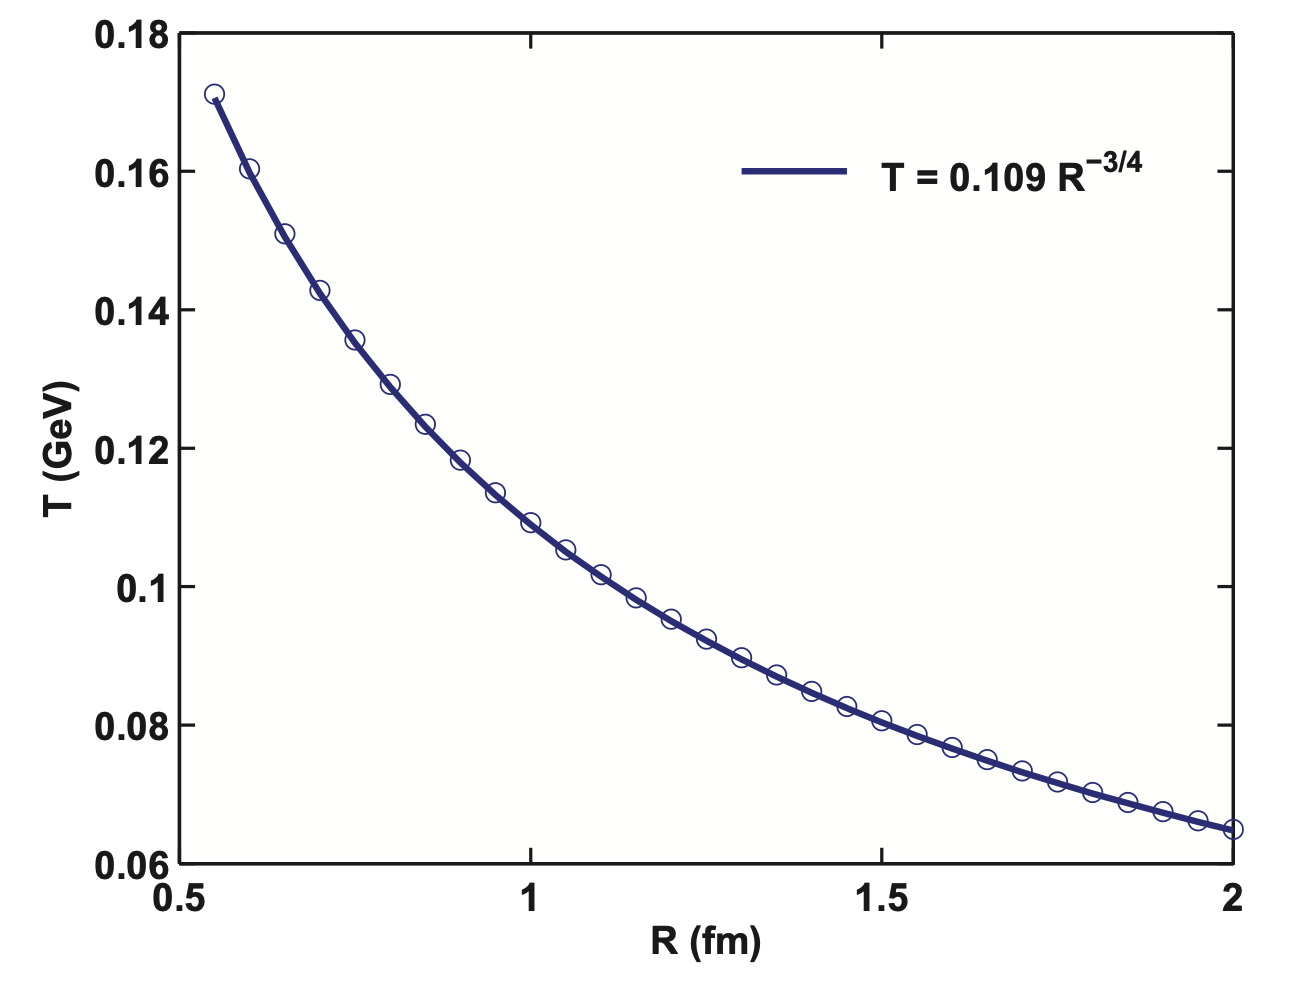
\includegraphics[width=0.5\textwidth]{./Images/T(R).png}
% \caption[Temperatura como función del radio del protón]{\emph{Ajuste realizado a una simulación numérica de la temperatura dentro del protón como función del radio}}
% \label{fig: T(r)}
% \end{wrapfigure}

% Tomando la masa de un nucleón como la energía total ${E}_{t} = M$, y siendo este como un sistema local en equilibrio térmico y despreciando el potencial químico, podemos calcular los cambios de temperatura con el radio del protón. De acuerdo con [Some characteristic parameters], se tiene una fórmula simulada numéricamente para la temperatura en función de la distacia al centro del protón, $r$, como 

% \begin{equation}\label{eq-T(r)}
% T = 0.109\left[ \frac{\unit{GeV}}{\unit{\femto\meter}}\right] {r}^{-3/4}, \quad (r  \text{ en \unit{\femto\meter}})
% \end{equation}

% A alrededor de $1 \, \mathrm{\unit{\femto\meter}}$, la temperatura es alrededor de $105 \, \mathrm{MeV}$. Cuando el radio de un protón es menor de $0.6 \, \mathrm{\unit{\femto\meter}}$, la temperatura probablemente será aproximada a $170 \, \mathrm{MeV}$, cercana a la temperatura crítica a la que el hadron se rompe a quarks.

% \begin{wrapfigure}{r}{0.4\textwidth}
% \centering
% 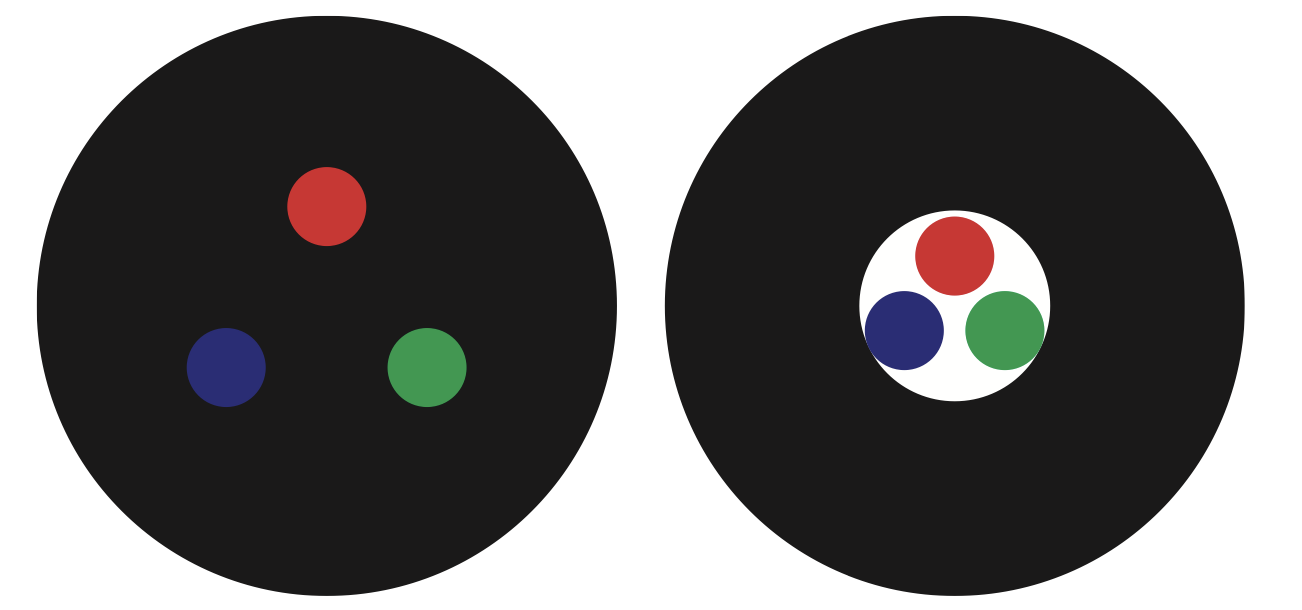
\includegraphics[width=0.4\textwidth]{./Images/Bag model-two scenaries.png}
% \caption[Posibles estructuras del modelo de bolsa]{
%  \emph{Tenemos dos posibilidades, i) que los quarks estén inmersos en un mar de gluones (izquierda) o ii) que los quarks estén \textbf{rodeados} \allowbreak por un mar de gluones(derecha)}}
% \label{fig: 2Bag-models}
% \end{wrapfigure}

% %\section*{Presión de bolsa como función de la distancia al centro del protón}

% Como vimos antes, en el capítulo \ref{ch-BagModel}, las soluciones a la ecuación \eqref{eq-condeigenval}, nos dan los límites de los radios de los hadrones considerando la relación ${\omega}_{n\kappa} = {p}_{n\kappa}{R}$, tenemos que para el estado más bajo accesible del sistema (que notaremos como ${\omega}_{1 \, -1} = {\omega}_{0} = 2.04$) y así para un protón, tenemos que la máxima energía cinética accesible para los quarks y gluones en el interior está dado por

% \begin{equation}\label{eq-maxp}
% {{p}_{0}}_{m} = \frac{2.04}{R}
% \end{equation}

% Si tomamos ${{p}_{0}}_{m}$ como el límite superior, podemos separar la energía de quarks del total de un protón

% \begin{equation}
% {E}_{Q} = \frac{\left({g}_{Q} + {g}_{\bar{Q}} \right) V}{2{\pi}^{2}{\hbar}^{3}} \int_{0}^{{{p}_{0}}_{m}} \frac{{p}^{3} \mathrm{d}p}{1 + {e}^{p/T(r)}}
% \end{equation}

% Por simplicidad, despreciamos el potencial químico, $\mu=0$, tratamos los quarks como sin masa y ${g}_{Q} = {g}_{\bar{Q}} = {N}_{c}{N}_{s}{N}_{f} = 3 \times 2 \times 2 = 12$, con ${N}_{c}$ es el número de colores (3 colores disponibles), ${N}_{s}$ el número de espín (2 espínes accesibles), y ${N}_{f}$ es el número de sabores (2 por ser \emph{up} y \emph{down}).


% La energía de contribución de gluones proporciona el efecto de presión dirigido desde fuera de la bolsa dada por

% \begin{equation}
% B = \frac{{E}_{t} - {E}_{Q}}{V}
% \end{equation}

% Existen dos posibles escenarios como se muestra en la figura \ref{fig: 2Bag-models}, el volumen del gas de gluones es ya sea $\frac{4 \pi}{3} {R}^{3}$ o $\frac{4\pi}{3}{R}_{i}^{3}$.

% \begin{wrapfigure}{l}{0.58\textwidth}
% \centering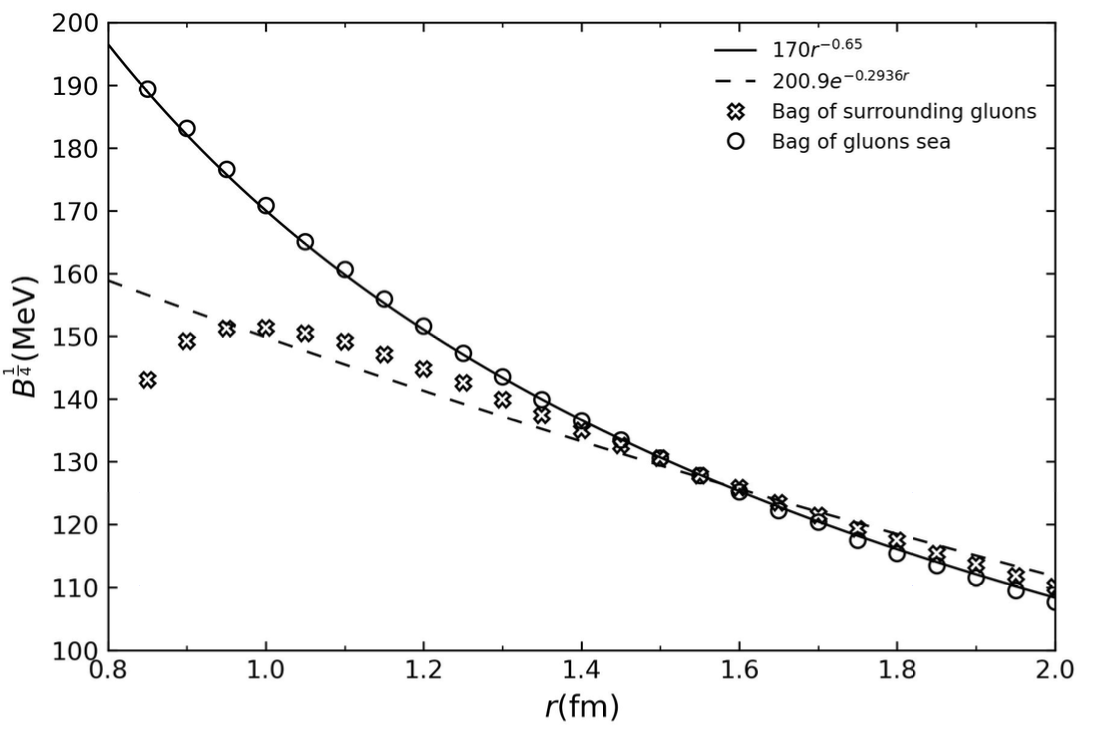
\includegraphics[width=0.58\textwidth]{./Images/B(R).png}

% \caption[Presión de bolsa como función del radio del protón]{\emph{Ajuste realizado a una simulación numérica de la presión de bolsa dentro del protón como función del radio. Tenemos dos posibles escenarios: El primero (representado por las cruces) considera a los quarks rodeados por un mar de gluones, mientras que el segundo (círculos) considera a los quarks en un mar de gluones. []}}
% \label{fig: B(r)}
% \end{wrapfigure}

% A partir del hecho de que la presión de bolsa depende del volumen de la misma, podemos pensar que la presión de bolsa cambiara con el radio (como se muestra en la figura \eqref{fig: B(r)}). Se pueden obtener los ajustes a ambos casos (el ajuste polinomial es el que mejor coeficiente de correlación obtiene para el caso de un mar de gluones), 

% \begin{equation}\label{eq-B(r)-seagluons}
% {B}^{1/4} = 0.17 \left[\frac{\unit{GeV}}{\unit{\femto\meter}}\right] {r}^{-0.65}
% \end{equation}

% o un ajuste exponencial para el \allowbreak segundo caso, gluones rodeando quarks, que obtiene, de entre \allowbreak varios otros ajustes (lineal, exponencial, \allowbreak logarítmico, polinomial) el mejor \allowbreak coeficiente de correlación

% \begin{equation}\label{eq-B(r)-gluonssorrounding}
% {B}^{1/4} = 0.201  {e}^{-0.293\left[\frac{1}{\unit{\femto\meter}}\right]r} \left[{\unit{GeV}}\right]
% \end{equation}

% Como una primera aproximación, usamos una presión de bolsa que es finita al centro del hadron y se desvanece a grandes distancias. Para este propósito, hemos determinado que una aproximación ajustable para la presión de bolsa es una exponencial de la forma \eqref{eq-B(r)-gluonssorrounding}, esta expresión, contiene el comportamiento que deseamos y esperamos para lo que sucede en el centro del hadrón, que en el centro la presión de la bolsa sea finita pero para grandes distancias se desvanezca.

----
\section{Derivación de la presión de quarks}\label{app:quark-pressure}

\subsection{Solución de la ecuación integral}
Aplicando la transformada inversa a \eqref{eq:d1-integral}:

\begin{equation}
p(r) = -\frac{k_p}{2\pi^2 r}\frac{d}{dr}\int_0^\infty x\,d_1(-x^2)\sin(rx)\,dx
\end{equation}

Sustituyendo \eqref{eq:d1-param}:

\begin{equation}
p(r) = \frac{k_p M^6 d_1(0)}{16\pi} e^{-Mr}\left(3 - Mr\right)
\end{equation}

\subsection{Normalización}
La constante $k_p$ se determina imponiendo \eqref{eq:stability}:

\begin{equation}
\int_0^\infty e^{-Mr}(3 - Mr)r^2 dr = 0 \quad \text{(Se cumple idénticamente)}
\end{equation}

El valor $k_p = 55$ se fija para reproducir:
\begin{itemize}
    \item El pico de presión $p(0) \approx \qty{0.35}{GeV/\femto\meter\cubed}$ de \cite{Burkert_2018}
    \item La transición a $p(r) < 0$ en $r \approx \qty{0.6}{fm}$
\end{itemize}

El factor $k_p \approx 55$ encapsula:
\begin{itemize}
    \item Efectos de orden superior no incluidos en $d_1(t)$
    \item Correlaciones quark-quark residuales
\end{itemize}